\documentclass[tikz,border=10pt]{standalone}
\usepackage{tikz}
\usetikzlibrary{arrows.meta,positioning}

\tikzset{
  box/.style={draw=blue!70!black, line width=1.2pt, rectangle, rounded corners=2pt, minimum width=3.0cm, minimum height=1.15cm, align=center, fill=none},
  signal/.style={->, line width=1.2pt, draw=black!80, >=Stealth}
}

\begin{document}
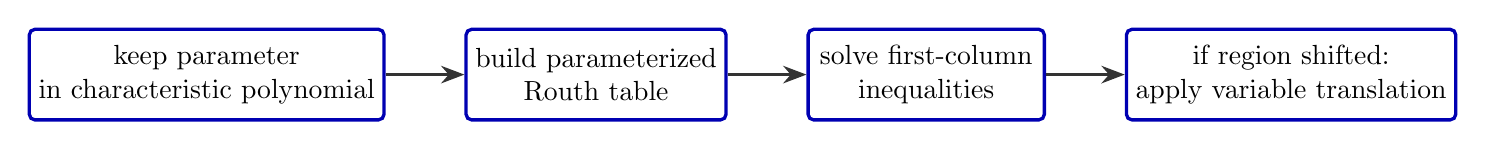
\begin{tikzpicture}[node distance=1.0cm]
  \node[box] (a) {keep parameter\\in characteristic polynomial};
  \node[box, right=of a] (b) {build parameterized\\Routh table};
  \node[box, right=of b] (c) {solve first-column\\inequalities};
  \node[box, right=of c] (d) {if region shifted:\\apply variable translation};
  \draw[signal] (a) -- (b);
  \draw[signal] (b) -- (c);
  \draw[signal] (c) -- (d);
\end{tikzpicture}
\end{document}
